\pagestyle{fancy}
%\newpage
\chapter{PSI: PLANIFICACIÓN DEL SISTEMA DE INFORMACIÓN}

	\vspace{2cm}	
	\begin{center}
	{\Large \textbf{FASE DE PLANIFICACIÓN} \par}
	\end{center}
	\vspace{5cm}
	
	\begin{center}
	\Huge \textbf{PSI}\par
	\end{center}

\newpage

\section{PSI 1: INICIO DEL PLAN DE SISTEMAS DE INFORMACIÓN}

\subsection{PSI 1.1: Análisis de la Necesidad del PSI} 
La creación de un museo de la historia de la informática es algo que da valor a la importancia de nuestra profesión y muestra el desarrollo que ha tenido esta disciplina en un corto espacio de tiempo. El tutor de este trabajo de fin de grado, José Manuel Redondo, tiene pensado crear con el tiempo un museo en esta línea, si bien por limitaciones de tiempo y recursos inicialmente lo ha limitado a CPUs. La crisis sanitaria del COVID-19 ha puesto los planes de seguir desarrollando un museo físico en pausa temporalmente, si bien se siguen recogiendo materiales con el objeto de que no acaban destruidos para ser expuestos en el futuro.\par
Debido a estas razones, y a la falta de por el momento del tiempo necesario para seguir desarrollando la iniciativa física, el tutor del proyecto ha propuesto el desarrollo de una aplicación web para el Museo de la Informática de Asturias, que contenga toda la información disponible sobre los componentes del museo (por el momento CPUs) y la muestre de forma ordenada. Convertir este museo, cuya primera versión está actualmente en exposición en la Escuela de Ingeniería Informática, a una aplicación web permitirá a más gente acceder a la información, y facilitará la exposición de nuevas piezas, ya que se reducirá el coste en recursos y tiempo, y no dependerá del espacio físico disponible en la Escuela o de su posible traslado al campus del Cristo. El sistema será gestionado directamente por el tutor del trabajo.
\par El sistema debe identificar cada componente y mostrar la información disponible del mismo. El software permitirá añadir la información de las nuevas piezas que puedan ser incluidas en la exposición en un futuro gracias a donaciones o compras. Los componentes serán ordenados según su tipo y la época a la que pertenecen. 

\subsection{PSI 1.2: Identificación del Alcance del PSI}
Actualmente los carteles informativos sobre las piezas del museo se encuentran expuestos en la Escuela de Ingeniería Informática. Los objetivos de este proyecto son los siguientes:
\begin{itemize}
	\item Recopilar los datos disponibles de las piezas que se encuentran actualmente en el Museo e introducirlos en una base de datos.	
	\item Facilitar la exposición de nuevas piezas respecto al museo físico.
	\item Mostrar una linea temporal con los diferentes periodos a los que pertenecen los componentes del Museo. 
	\item Permitir acceder a cada periodo para ver los componentes del mismo.
	\item Organizar las diferentes piezas en función de su tipo y de la familia de la que forman parte.
	\item Presentar la información disponible de cada pieza, así como imágenes de la misma y otras curiosidades.
\end{itemize}
En definitiva, estos objetivos se pueden resumir en:
\begin{itemize}
	\item Permitir a los usuarios visitar el Museo de la Informática de forma online, ofreciendo la misma información que se encuentra disponible en la exposición física.
	\item Facilitar al administrador la inserción de nuevos periodos y componentes.
\end{itemize}

\subsection{PSI 1.3: Determinación de Responsables}
\begin{itemize}
	\item \textbf{El proyectante} se encargará del desarrollo del software descrito y de realizar la carga de los datos disponibles a la base de datos correspondientes.
	\item\textbf{El tutor del proyecto} se encargará de la supervisión de las fases del proyecto y de su validación.
	\item \textbf{Una serie de usuarios escogidos aleatoriamente} realizará pruebas del software para comprobar su correcto funcionamiento.
\end{itemize}


%\newpage
%\section{PSI 2: DEFINICIÓN Y ORGANIZACIÓN DEL PSI}
% 
%
%\subsection{PSI 2.1: Especificación del Ámbito y Alcance} 
%
%
%\subsection{PSI 2.2: Organización del PSI}


%\newpage
%\section{PSI 3: ESTUDIO DE LA INFORMACIÓN RELEVANTE}
% 
%\subsection{PSI 3.1: Selección y Análisis de Antecedentes} 


\newpage

\section{PSI 7: DEFINICIÓN DE LA ARQUITECTURA TECNOLÓGICA}
%\subsection{PSI 7.1: Identificación de las Necesidades de Infraestructura Tecnológica} 


\subsection{PSI 7.2: Selección de la Arquitectura Tecnológica}\label{sec:arq-tec}
La aplicación seguirá la arquitectura Modelo Vista Controlador (MVC), patrón arquitectónico que separa los datos y la lógica de una aplicación de su representación. Esta elección se debe a que el MVC es uno de los modelos más conocidos en la arquitectura web.
\begin{itemize}
\item El modelo es la capa que trabaja con los datos.
\item La vista permite la visualización de los datos con los que trabaja el modelo.
\item El controlador es una capa que enlaza la vista y el modelo.
\end{itemize}
\par Será alojada en las máquinas de la universidad disponibles para estos proyectos, una máquina Linux con Apache y MySQL.
\begin{figure}[H]
\vspace{4mm}
\centering
\centerline{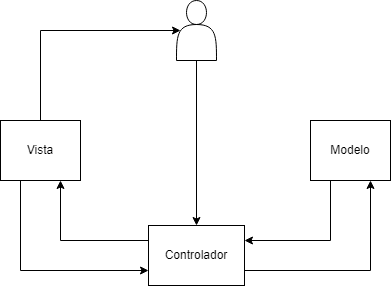
\includegraphics[scale=0.6]{mvc}}
\caption{Arquitectura MVC}
\end{figure}